\chapter{Simulations}
\label{simulation}
As mentioned in Chapt.~\ref{chapt:kin} there are important processes that contribute to the overall $Q$-value resolution that are random in nature.  These random contributions, which include target thickness effects and detector resolution, are important when assessing the feasibility of using the HELIOS spectrometer to measure a given reaction.  Monte Carlo simulations are performed to characterize the realistic response of HELIOS; these simulations %are similar to those described 
appear in Refs.~\cite{Wuosmaa_2007} and \cite{Lighthall_2010}.  The latter incorporates tracking of particles through the actual measured field map of the HELIOS solenoid, and a detector array with dimensions of the actual array.  The simulations appearing in these references both use the method described below.  

\section{Method}
Three separate programs, all based on C++ code, are used to generate the simulations which model the performance characteristics of HELIOS.    The first program is a kinematics program which takes as an input the reaction being studied, the bombarding energy of the beam and the excitation states of interest.  Also input are the range of angles over which the reaction product are emitted and the thickness of the target.  Using the principles of two-body kinematics as described in Chapt.~\ref{chapt:kin}, this program generates initial trajectories of the reaction products.  For each trajectory, the program randomly generates the emission angle $\theta_\mathrm{lab}$ (within the specified range) and calculates the energies of the reaction products.  The results of this step of the simulation are equivalent to the analytic calculations  shown in Fig.~\ref{sn-plots}.  Part of the output of this program is a randomly generated azimuthal emission angle $\phi$ and interaction depth within the target.  

The initial trajectories produced by the first program serve as the input for the second program which tracks the particle trajectories through HELIOS.  The features that distinguish the particle tracking simulation from analytical calculations are the inclusion of target thickness effects, beam spot size, and realistic detector resolution.  Each of these contributions have a random component and are thus best calculated in a Monte Carlo simulation.  In addition, tracking the particles through the real magnetic field map, and using realistic detector geometry lend themselves to iterative calculation.  To run a simulation, a list of parameters is used to specify the physical dimensions and characteristics of the solenoid and the detector arrays.  Most of these parameters remain constant; the ones that are typically changed for each simulation are the magnetic field strength $\mathscr{B}_0$ and the position of the detector arrays.  

Particle tracking begins in the target.  The simulation uses the interaction depth with the target to calculate energy loss and multiple scattering. Then a position within the beam spot is randomly generated and the new starting trajectory---a position and velocity vector---is passed to the tracking simulation.  At each point in tracking  the particle trajectory $\vec{r}_{n}$, the value of the magnetic field is interpolated from the field map $\mathscr{B}(\vec{r}_{n})$, where $n$ is the iteration step.  Interpolation algorithms of varying sophistication can be used; a linear interpolation based on the values listed in Appendix~\ref{field_map_data} is used in the simulations appearing in this document.  At each iteration step in the particle tracking, the components of the radius and velocity vectors are calculated as

\begin{subequations}
\label{sim_setp}
\begin{eqnarray}
(v_i)_n=\left[\vec{v}_{n-1} \times \mathscr{B}(\vec{r}_{n-1})\right] \frac{q}{m}dt \label{r_step}\\
(r_i)_n=(v_i)_n dt \label{v_step}
\end{eqnarray}
\end{subequations}
where the quantity in the square brackets is the acceleration due to the magnetic field and $i$ can be $x$, $y$, or $z$.
A typical value of the time step used in the simulation is 0.02\,ns, corresponding to about 1,500 tracking iterations before a successful particle detection.  Tracking terminates if the particle hits the solenoid bore, intercepts the detector array, or exits the end of the solenoid.

Finally, the output of the tracking simulations are histogramed using ROOT~\cite{Brun_1998}.  For the simulated spectra appearing in this document (and in Refs.~\cite{Wuosmaa_2007, Lighthall_2010}), the histograms are produced in a manner very similar to those made with  experimental data.  That is, the simulated energy and position signals from each simulated detector are used to generate the histograms. 

\section{Results}
\begin{figure}[ht]
	\centering
	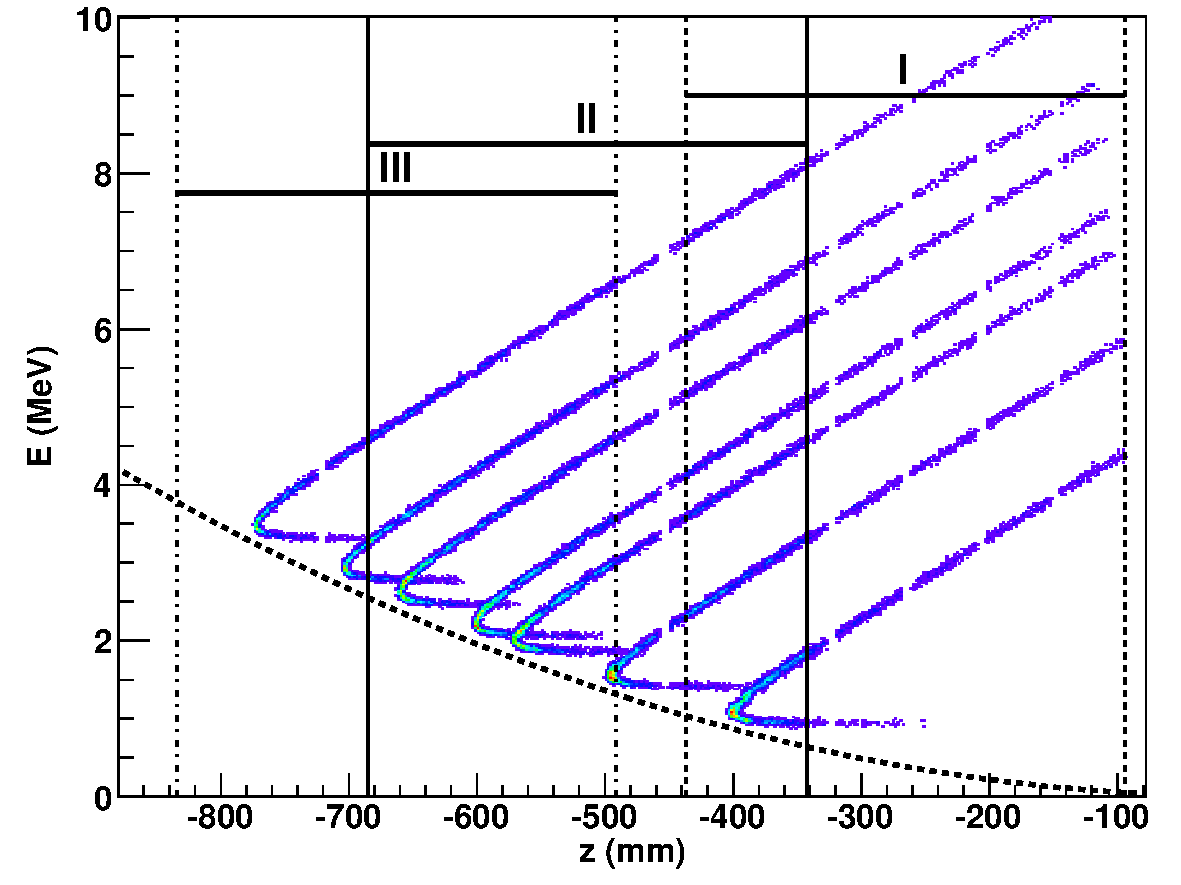
\includegraphics[width=\linewidth,keepaspectratio]{../NIM_Paper/Figures/cSim}
	\caption[Simulated $E_\mathrm{lab}$ vs. $z$ spectrum from the $d$($^{28}$Si,$p$)$^{29}$Si reaction with HELIOS]{Simulated $E_\mathrm{lab}$ vs. $z$ spectrum from the $d$($^{28}$Si,$p$)$^{29}$Si reaction with HELIOS.  Seven states in $^{29}$Si are plotted using the field map of the actual HELIOS solenoid.  Pairs of vertical lines indicate the length of the array coverage with leading edges at $-94$\,mm, $-342$\,mm, and $-492$\,mm.  %The wide-dashed line indicating the high-energy cutoff is due to particles intercepting the solenoid bore.
	The narrow-dashed line indicating the low-energy cutoff is due to particles intercepting the front of the detector array. This figure also appears in Ref.~\cite{Lighthall_2010}.}
\label{sim_plots}
\end{figure}

Fig.~\ref{sim_plots} shows a simulated spectrum of proton energy versus position for the $d$($^{28}$Si,$p$)$^{29}$Si reaction, calculated at three different target-detector separations.  The simulations assume uniform angular distributions, a CD$_2$ target thickness of 84\,$\mu$g/cm$^2$, and an energy resolution of 50\,keV~FWHM.  The simulation does not include detector threshold effects.  The vertical gaps in the spectrum are due to the spacing between detectors on the array.  The simulated response of the spectrometer shown in Fig.~\ref{sim_plots} is ostensibly  identical to the analytic calculations shown in Fig.~\ref{analytic}.  For this set of simulations, the particle trajectories probe the central region of the solenoid where the magnetic field is most uniform.  The effect of field non-uniformities on peripheral trajectories is discussed below.  As previously mentioned, an important difference between the analytic calculations and the simulations is the ability to study the realistic excitation energy resolution.  Fig.~\ref{sim_res} shows the effect that the realistic magnetic field has on the excitation energy resolution as compared to a simulation assuming an ideal (uniform) magnetic field.  For this pair of simulations, the target is located at the center of the magnet ($z$=0) and the silicon detector array is positioned upstream at $\Delta z = 94\,$mm.  With this experimental setup, the target, the entire array, and all of the particle orbits are confined to the 90\,cm~DSV of greatest field uniformity.  Both simulations assume 50\,keV detector resolution, 1\,mm$^2$ beam spot size, and the target effects from a 84\,$\mu$g/cm$^2$ thick  CD$_2$ target.

\begin{figure}%
\centering
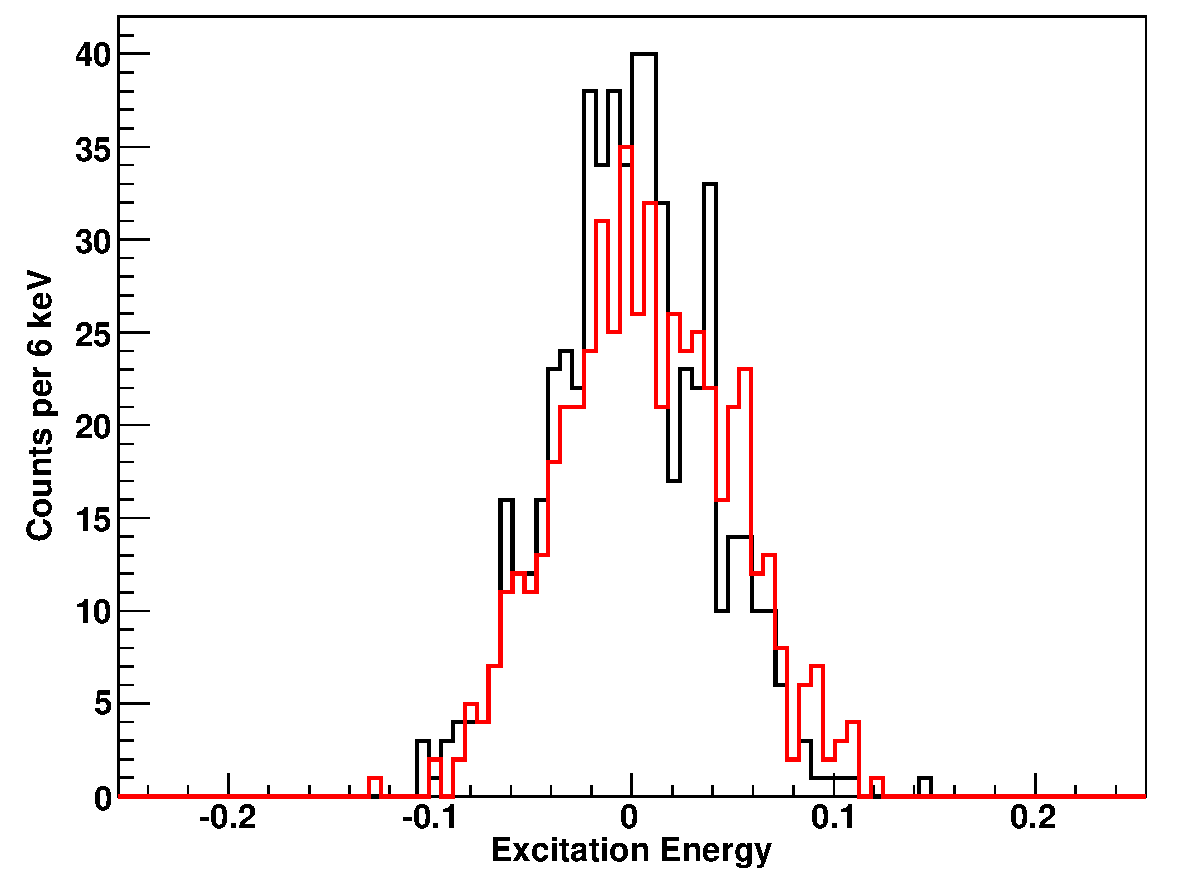
\includegraphics[width=\columnwidth,height=0.33\textheight,keepaspectratio]{csimQ}%
\caption[Simulated $Q$-value resolution of the ground state of $^{29}$Si using realistic parameters]{(color online) Simulated $Q$-value resolution of the ground state of $^{29}$Si using realistic parameters.  The simulation producing the black histogram assumes an ideal magnetic field; the width of the peak is 89.6\,keV~FWHM.  The gray (red) histogram is produced using the measured field map; the width of the peak is 100.0\,keV~FWHM.  Based on these and other simulations, the average contribution of the realistic magnetic field 48.7\,keV (which gets added in quadrature to the other contributions).}%
\label{sim_res}%
\end{figure}

Following the method illustrated in Fig.~\ref{sim_res}, several pairs of simulations were run, changing one simulation parameter in each pair.  The results of the $Q$-value analysis of these simulations are shown Table~\ref{sim_prop}.  Neglecting the beam spot size, target thickness effects, and the non-uniformity of the magnetic field, Table~\ref{helios_error} shows that the $Q$-value resolution should be dominated by the intrinsic detector resolution; as is the case in normal kinematics.  However, in inverse kinematics, due to the heavy ion reactant being the particle which passes through the target foil, Table~\ref{sim_prop} shows that even for a relatively thin target, target thickness effects are significant---on the order of 35\,keV.  The simulations also show that careful alignment of the silicon detector array and a well-defined beam are also important.  A 1\,mm$^2$ beam spot size, or equivalently, a $\pm0.5$\,mm beam misalignment contributes over 60\,keV to the $Q$-value resolution; this contribution is greatest in the region of the knees.  Finally, the contribution of the measured magnetic field in the central region of the solenoid is on the order of the intrinsic detector resolution, about 49\,keV.  All of these contributions get added in quadrature, according to the law of error propagation~\cite{Bevington_2003,Drosq_2007}.

\begin{table*}%
  \centering
  \begin{tabular}{,.d{1}d{1}d{1}d{1}d{1}r}		
    \hline
    \multicolumn{1}{c}{\multirow{2}{*}{Reaction}}  &
    \multicolumn{1}{c}{$E_1/A_1$}  &
    \multicolumn{1}{c}{$\mathscr{B}$} & 
    \multicolumn{4}{c}{Origin of contribution}  &
    \multicolumn{1}{c}{$\delta E_\textrm{cm}$}  \\  \cline{4-7}
    &\multicolumn{1}{c}{(\AMeV)}&
    \multicolumn{1}{c}{(T)} & 
    \multicolumn{1}{c}{PSD}  &  
    \multicolumn{1}{c}{beam}  &  
    \multicolumn{1}{c}{target} & 
    \multicolumn{1}{c}{field} & 
    \multicolumn{1}{c}{$\Sigma_\mathrm{quad}$} \\
    \hline \hline 
		d(^{28}\textrm{Si},p)^{29}\textrm{Si} 	 &6.02 & 2.00 &50.0&65.4& 35.3 &48.7 &102.0  \\
%		d(^{12}\textrm{B},p)^{13}\textrm{B} 	 &6.24 & 155.2 &25 & 93 & 7 & 97 & 118\\
%		d(^{132}\textrm{Sn},p)^{133}\textrm{Sn}	 &4.78 & 149.0 &22 & 111 & 7 & 113 & 133\\
%		d(^{124}\textrm{Sn},^3\textrm{He})^{123}\textrm{In} 	 &13.00 & 21.5 &87 & 72 & 55 & 126 & 57\\
%		p(^{77}\textrm{Kr},d)^{76}\textrm{Kr}  	 &30.00 & 15.1 &118 & 54 & 85 & 156 & 106\\
		\hline
  \end{tabular}
  \caption[Derived contributions  to the uncertainty $E_\textrm{cm}$ based on Monte-Carlo simulations]{Derived contributions to the uncertainty of the center-of-mass energy $E_\textrm{cm}$ based on Monte-Carlo simulations.  Values are determined based on a 50\,keV~FWHM detector resolution (PSD), 1\,mm$^2$ beam spot size (beam), a CD$_2$ target 84\,$\mu$g/cm$^2$ thick (target), and the measured field map (field).  The quadratic sum $\Sigma_\mathrm{quad}$ is equal to the simulated $Q$-value resolution.}
  \label{sim_prop}
  \end{table*}

Fig.~\ref{sim_bad} shows the simulated proton spectrum for the $d$($^{28}$Si,$p$) reaction with the silicon detector array placed as far upstream as it will move, with the leading edge (target-end) of the active area of the silicon detectors placed at $z=-396$\,mm.  Two target-to-detector settings are shown, $\Delta z=100$\,mm and $\Delta z=450$\,mm to mimic the detector coverage of the $d$($^{28}$Si,$p$) measurement.  Analytic calculations of the locations of the protons groups have been plotted over the simulations for comparison.  It is clear that simulated protons detected at the $\Delta z=100$\,mm setting have had their orbits altered by the inhomogeneities of the magnetic field.

Fig.~\ref{sim_traj} shows calculated proton trajectories for the two target-to-array settings used to produce the simulation.  Trajectories have been calculated for the ground state transition to $^{28}$Si.  Taking $T_\mathrm{cyc}$, $v_\parallel$, and $r$ as inputs, Eqs.~\ref{eq:rot} and \ref{eq:radius} are used to plot the radial excursion $p$ as a function of $z$.  At each target position six trajectories are plotted, each intercepting the center of a detector element.  
Setting I ($\Delta z=100$\,mm) corresponds to emission angles of  $\theta_\mathrm{lab}=95^\circ$--110$^\circ$ and orbit excursions of $\rho=37$--46\,cm.  Setting II ($\Delta z=450$\,mm) corresponds to emission angles of  $\theta_\mathrm{lab}=114^\circ$--158$^\circ$ and orbit excursions of $\rho=10$--34\,cm.  Inspection of Figs.~\ref{sim_bad} and \ref{sim_traj} shows that the distortions due to the magnetic field are greatest for orbits with the greatest radial excursion.  Comparing Figs.~\ref{sim_plots} and \ref{sim_bad} shows that this negative effect is absent for orbits in the center of the solenoid.

Despite the deformation of the spectrum, two important features should be recognized.  First, by inspection, the spacing of the kinematic groups remains constant, even for particles whose orbits probe the regions of more non-uniform magnetic field.  The dependence of energy on position is not precisely linear, however the separation in energy between different kinematic groups is retained.  Therefore, the performance of the spectrometer as defined by $Q$-value resolution is not adversely effected by the field non-uniformities.  The second important feature to note is that the simulated protons groups measured at the $\Delta z=100$\,mm setting---corresponding to orbits with smaller radii ($r<17.5$\,cm)---exhibit almost no deformity.  The conclusion to be drawn from this observation is that the fiducial volume for small orbit radii ($r<17.5$\,cm) extends over the entire length solenoid which is within the acceptance of the array ($|z|<74$\,cm).  In this region, the mean absolute field non-uniformity is 0.67\%.  It is also interesting to note that the $z=-396$\,mm silicon detector array setting is nearly the same  position used in the $^{11,12}$B($d$,$p$) experiment which exhibits no field-induced deformities in the shape of the kinematic loci (see Fig.~\ref{b11_spec}).
 
\begin{figure}
\centering
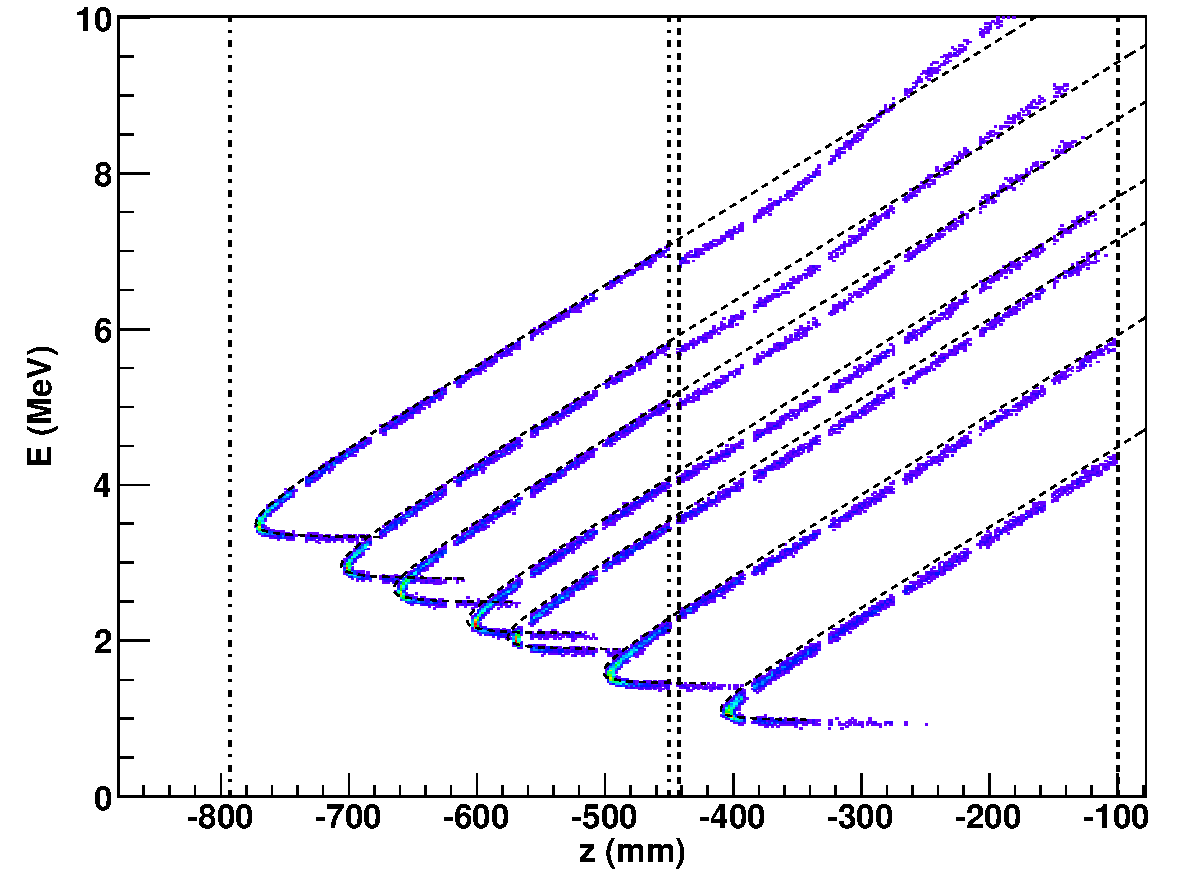
\includegraphics[width=\columnwidth]{csimB}%
\caption[Simulated proton spectrum showing distortions due to field inhomogeneities]{Simulated proton spectrum showing distortions due to field inhomogeneities.  The $d$($^{28}$Si,$p$) reaction is simulated with the detector array at $z=-396$\,mm (furthest possible upstream position).  Two target-to-detector settings are shown, $\Delta z=100$\,mm and $\Delta z=450$\,mm.  Distortions due to field inhomogeneities are more pronounced for orbits with larger radii ($\Delta z=100$\,mm setting).  The apparent discontinuity between the data sets is due protons probing different regions of the magnetic field for the two different target-to-detector settings.  Refer to Fig.~\ref{sim_traj} for an illustration of the particle trajectories.}%
\label{sim_bad}%
\end{figure}

\begin{figure}%
\centering
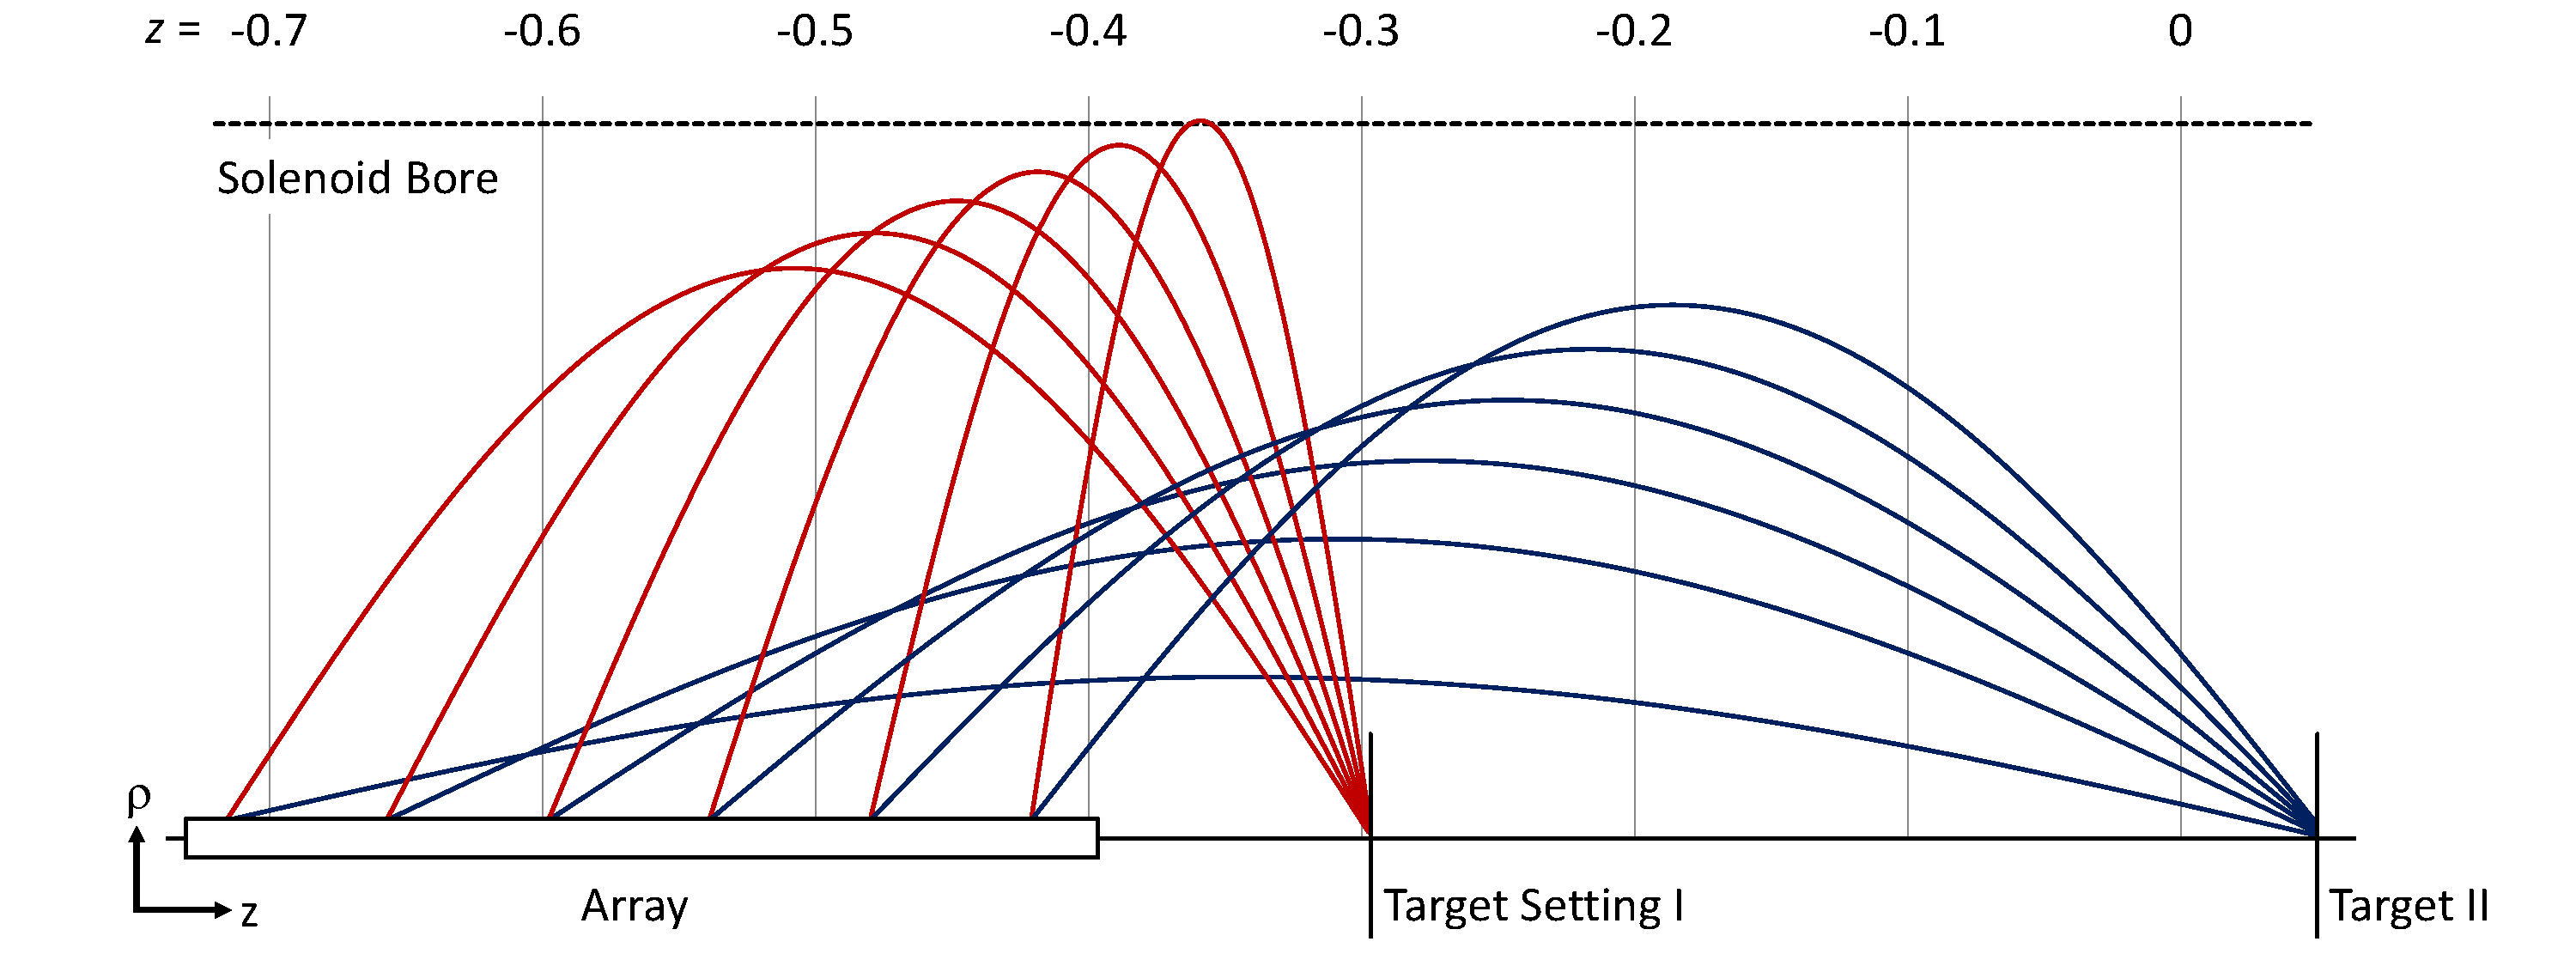
\includegraphics[width=\columnwidth]{sim_traj}%
\caption[Calculated proton trajectories from $d$($^{28}$Si,$p$) for two different target-to-detector settings]{Calculated proton trajectories from $d$($^{28}$Si,$p$)  for two different target-to-detector settings.  Separations of $\Delta z=100$\,mm and $\Delta z=450$\,mm are shown, with the silicon detector array positioned at $z=-396$\,mm.  Drawn to scale.}
\label{sim_traj}%
\end{figure}